% !TeX spellcheck = en_US
\documentclass[a4paper]{scrartcl}
\usepackage{graphicx}
\usepackage{listings}
\usepackage{color}
\usepackage{amsmath}

\definecolor{mygreen}{rgb}{0,0.6,0}
\definecolor{mygray}{rgb}{0.5,0.5,0.5}
\definecolor{mymauve}{rgb}{0.58,0,0.82}

\lstset{ 
	backgroundcolor=\color{white},   % choose the background color; you must add \usepackage{color} or \usepackage{xcolor}; should come as last argument
	basicstyle=\tiny,        % the size of the fonts that are used for the code
	breakatwhitespace=false,         % sets if automatic breaks should only happen at whitespace
	breaklines=true,                 % sets automatic line breaking
	captionpos=b,                    % sets the caption-position to bottom
	commentstyle=\color{mygreen},    % comment style
	deletekeywords={...},            % if you want to delete keywords from the given language
	escapeinside={\%*}{*)},          % if you want to add LaTeX within your code
	extendedchars=true,              % lets you use non-ASCII characters; for 8-bits encodings only, does not work with UTF-8
	frame=single,	                   % adds a frame around the code
	keepspaces=true,                 % keeps spaces in text, useful for keeping indentation of code (possibly needs columns=flexible)
	keywordstyle=\color{blue},       % keyword style
	language=Octave,                 % the language of the code
	morekeywords={*,...},            % if you want to add more keywords to the set
	numbers=left,                    % where to put the line-numbers; possible values are (none, left, right)
	numbersep=5pt,                   % how far the line-numbers are from the code
	numberstyle=\tiny\color{mygray}, % the style that is used for the line-numbers
	rulecolor=\color{black},         % if not set, the frame-color may be changed on line-breaks within not-black text (e.g. comments (green here))
	showspaces=false,                % show spaces everywhere adding particular underscores; it overrides 'showstringspaces'
	showstringspaces=false,          % underline spaces within strings only
	showtabs=false,                  % show tabs within strings adding particular underscores
	stepnumber=1,                    % the step between two line-numbers. If it's 1, each line will be numbered
	stringstyle=\color{mymauve},     % string literal style
	tabsize=2,	                   % sets default tabsize to 2 spaces
	title=\lstname                   % show the filename of files included with \lstinputlisting; also try caption instead of title
}
\begin{document}
	
	\title{Processor Microarchitecture}
	\author{Tim Burkert}
	
	\maketitle
	
	\begin{abstract}
		Report, results and evaluation of practical exercises done during Processor Microarchitecture lecture.
	\end{abstract}
	
	\section{Exercise Description}
	As a practial exercise three different testcases are given. For each testcase four assignments need to be fulfilled.
	
	\paragraph{Testcases}
	
	\begin{description}
		\item Color conversion \\
		RGB color to grayscale with following equation: \\
		$\textbf{intensity} = 0.29894*r + 0.58704*g + 0.11402*b$
		
		\item Histogram calculation \\
		Create a histogram with a given amount of bins for a set of values \\
		$\textbf{histogram[intensity(x,y)]} += 1, \forall (x,y) \in Image$
		
		\item Edge detection \\
		Applying sobel filter to an image \\
		$E(x,y) = I(x,y) * S(x,y)$
	\end{description}
	
	\paragraph{Assigments}
	
	\begin{description}
		\item Write the the program \\
		Experiment in octave \\
		Convert from octave to c \\
		
		\item Analyze classical in-order execution \\
		Compile C to SpartanMC and LEON3 assembly \\
		Analyze the used instructions from the assembly listing a statistics \\
		Profile the execution in ModelSim a statistics \\
		Based on the previous analyses suggest instruction set improvements \\
		
		\item Datapath construction \\
		Construct a statically scheduled pipeline for the computation in C \\
		Get the basic function units from Xilinx Coregen \\
		Verify the datapath in ModelSim against the reference data from C\\
		
		\item Analyze micro-threaded in-order execution \\
		Convert the C program to the SLC language or by hand to the microthreaded assembly. \\
		Execute in UTLEON3 – ModelSim, SP605 \\
		Profile execution in ModelSim, identify bottlenecks and restructure the program accordingly \\
	\end{description}
	
	\section{Color Conversion}
	Conversion form a 24 Bit rgb value to an 8 Bit grayscale value can be done with various precisions and methods. A example using double precision floats is given in octave \textit{rgb2gray}. This method uses a luminosity equation to compute the intensity for each pixel. We implemented the same equation using fixed point arithmetics. For this we firstly converted the luminosities factors for each color to 20 Bit integer value.
	\begin{align*}
		rf &= 0.29894_{10} \approx  0.01001100100001110101_{2} = 313461_{10} * 2^{-20} \\
		gf &= 0.58704_{10} \approx  0.10010110010010000100_{2} = 615556_{10} * 2^{-20} \\
		bf &= 0.11402_{10} \approx  0.00011101001100000111_{2} = 119559_{10} * 2^{-20} \\
	\end{align*}
	
	To test how different precisions for each factor perform we implemented a following octave function. The function takes an image and a 3x1 vector describing the bit precision for each factor from max 20 to 0. With this function we can test arbitrary bit length combinations.

\begin{minipage}{\linewidth}
\begin{lstlisting}
function [J] = ui8rgb2gray (I, bits)
rf = bitshift(uint64(313461), bits(1)-20);  # 0.01001100100001110101
gf = bitshift(uint64(615556), bits(2)-20);  # 0.10010110010010000100
bf = bitshift(uint64(119559), bits(3)-20);  # 0.00011101001100000111
uI = uint64(I);
for i = 1:rows(I)
	for j = 1:columns(I)
		r = rf * uI(i,j,1);
		g = gf * uI(i,j,2);
		b = bf * uI(i,j,3);
		J(i,j) = uint8(bitshift(r, -bits(1))) 
			+ uint8(bitshift(g, -bits(2))) 
			+ uint8(bitshift(b, -bits(3)));
	endfor
endfor
endfunction
\end{lstlisting}
\end{minipage}	

    \subsection{Error Evaluation}

	The total error of rgb to grayscale conversion is a combination of the indepandant transformation for each channel. The total worst case error is the sum of all three partial worst case errors. Therefore to decide how many bits precision are need for each color channel, we did an error evaluation of each channel. For this we used three different metrices: Maximum Difference, Maximum Weighted Difference and Root Mean Square Error (RMSE)

\paragraph{}
The Maximum Weigted Difference describes the error for a total converted image better then the other metrices. Because the total error of each channel doesnt effect the total error equal. The total error contribution is depends on the used conversion factors for each channel.
\begin{align*}
 \textbf{intensity} &= 0.29894*r + 0.58704*g + 0.11402*b
\end{align*}


Therefore the green channel twice the error contribution then the red channel and six times the contribution to the blue channel. Because this asymetric error contribution we choosed an asymetric bit precision for each channel. We used for the green channel 7 Bit precision conversion factor, red channel 6 Bit precision conversion factor and for the blue channel only a 5 Bit precision conversion factor.

\begin{figure}[h]
  \centering
  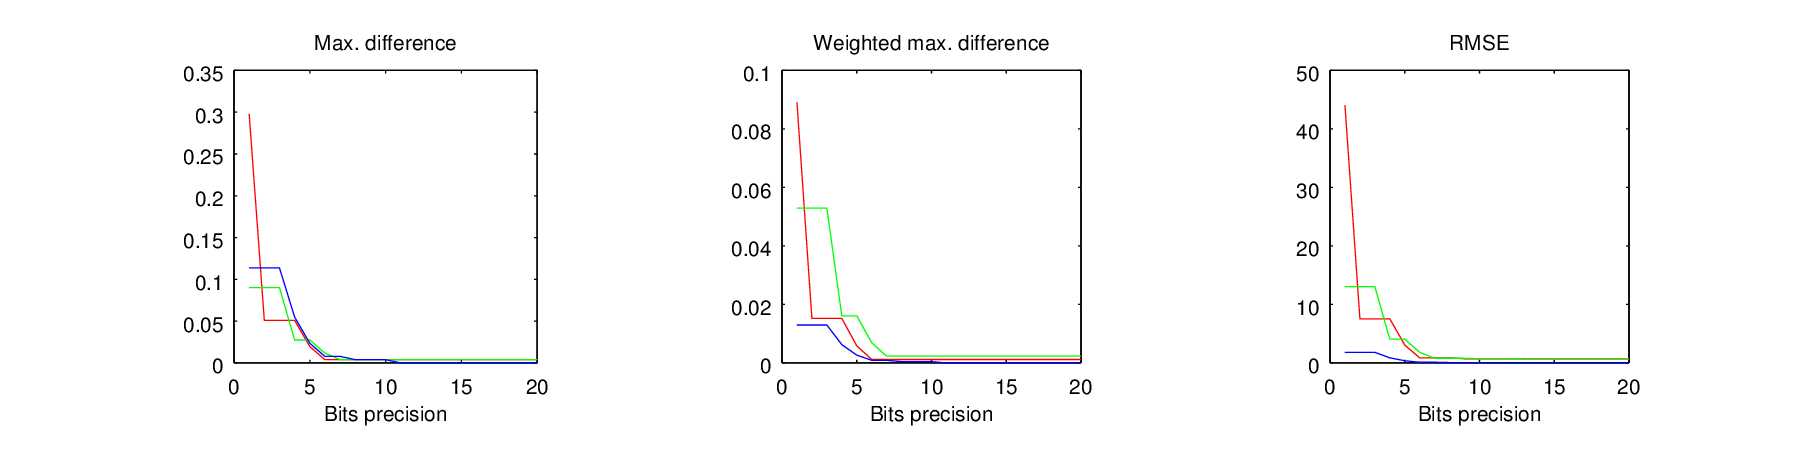
\includegraphics[width=\textwidth]{gray_error} 
  \caption{Maximum difference, weigthed maximum difference and RMS Error comparing octave rgb2gray and our implementation.}
\end{figure}


\end{document}